\newcommand{\partthreeabstract}{Two rounds of reference-guided diffusion with active view selection and geometric confidence increase PSNR by 0.007--0.041~dB over matched real-only continuation on the three course scenes and by 0.035~dB on an additional indoor scene. LPIPS also improves over that control. Compared with the initial sparse scenes, the second round gives modest PSNR gains and lower SSIM.}

\newcommand{\partthreeconclusion}{The closed loop gives small improvements over real-only continuation. Its advantage over ungated diffusion is under 0.006~dB in final PSNR, with a slight perceptual cost on the course scenes. These results suggest that wider training coverage and reliable camera geometry remain important even when a generator improves individual rendered views.}

\newcommand{\partthreeassets}{%
\begin{table*}[!t]
  \centering\small
  \setlength{\tabcolsep}{4.0pt}
  \begin{tabular}{llrrrrrrrrr}
    \toprule
    & & \multicolumn{3}{c}{Waymo-405841} & \multicolumn{3}{c}{Dl3dv-2} & \multicolumn{3}{c}{Re10k-1} \\
    \cmidrule(lr){3-5}\cmidrule(lr){6-8}\cmidrule(lr){9-11}
    Round & Condition & PSNR $\uparrow$ & SSIM $\uparrow$ & LPIPS $\downarrow$ & PSNR $\uparrow$ & SSIM $\uparrow$ & LPIPS $\downarrow$ & PSNR $\uparrow$ & SSIM $\uparrow$ & LPIPS $\downarrow$ \\
    \midrule
    0 & Sparse baseline & 16.7260 & 0.5971 & 0.4574 & 15.4786 & 0.4559 & 0.2572 & 11.2342 & 0.2751 & 0.4055 \\
    \midrule
    1 & Real only & 16.6996 & 0.5926 & 0.4535 & 15.4744 & 0.4540 & 0.2584 & 11.2339 & 0.2739 & 0.4063 \\
      & Raw replay & 16.7093 & 0.5936 & 0.4536 & 15.4856 & 0.4550 & 0.2576 & 11.2366 & 0.2742 & 0.4059 \\
      & Active + ungated & \textbf{16.7129} & \textbf{0.5947} & \textbf{0.4525} & 15.5180 & 0.4561 & \textbf{0.2549} & 11.2381 & \textbf{0.2749} & 0.4043 \\
      & Fixed + gated & -- & -- & -- & -- & -- & -- & \textbf{11.2415} & 0.2747 & \textbf{0.4038} \\
      & Active + gated & 16.7117 & 0.5945 & 0.4528 & \textbf{15.5201} & \textbf{0.4563} & 0.2555 & 11.2371 & 0.2745 & 0.4044 \\
    \midrule
    2 & Real only & 16.7040 & 0.5898 & 0.4524 & 15.4720 & 0.4531 & 0.2592 & 11.2434 & 0.2742 & 0.4066 \\
      & Raw replay & 16.6986 & 0.5910 & 0.4520 & 15.4872 & \textbf{0.4543} & 0.2579 & 11.2485 & \textbf{0.2748} & 0.4061 \\
      & Active + ungated & 16.7419 & \textbf{0.5928} & \textbf{0.4511} & 15.4955 & 0.4509 & \textbf{0.2575} & 11.2493 & 0.2744 & 0.4044 \\
      & Fixed + gated & -- & -- & -- & -- & -- & -- & 11.2459 & 0.2743 & \textbf{0.4043} \\
      & Active + gated & \textbf{16.7445} & 0.5925 & 0.4513 & \textbf{15.5009} & 0.4521 & 0.2579 & \textbf{11.2505} & 0.2746 & 0.4045 \\
    \bottomrule
  \end{tabular}
  \caption{Test metrics of the raw Gaussian renders. Round zero is the 7,000-step Part 2 checkpoint. Each subsequent round adds 3,000 matched real-image updates. Bold marks the best metric among evaluated conditions within a scene and round, before rounding. Fixed planning is evaluated on Re10k-1.}
  \label{tab:part3_main}
\end{table*}
\begin{figure*}[!t]
  \centering
  \includegraphics[width=0.93\textwidth]{active_trajectory.png}
  \caption{Sparse training cameras and the virtual views chosen for restoration. Each panel projects camera centers into its first two principal axes and uses its own scale. The active planner reranks candidates with the updated scene's alpha maps in round two.}
  \label{fig:active_trajectory}
\end{figure*}

\begin{figure*}[!t]
  \centering
  \includegraphics[width=0.93\textwidth]{closed_loop_psnr.png}
  \caption{Held-out PSNR change from the initial sparse model at each round. The panels use independent vertical ranges to show within-scene differences.}
  \label{fig:closed_loop}
\end{figure*}

\begin{figure*}[!t]
  \centering
  \includegraphics[width=0.93\textwidth]{pseudo_views.png}
  \caption{Two Re10k-1 virtual views before and after reference-guided diffusion, selected for highest verified support in round one and lowest verified support in round two. Each reference is a real sparse training view. The confidence map shows the pixel weights used by gated fusion.}
  \label{fig:pseudo_views}
\end{figure*}

\begin{figure*}[!t]
  \centering
  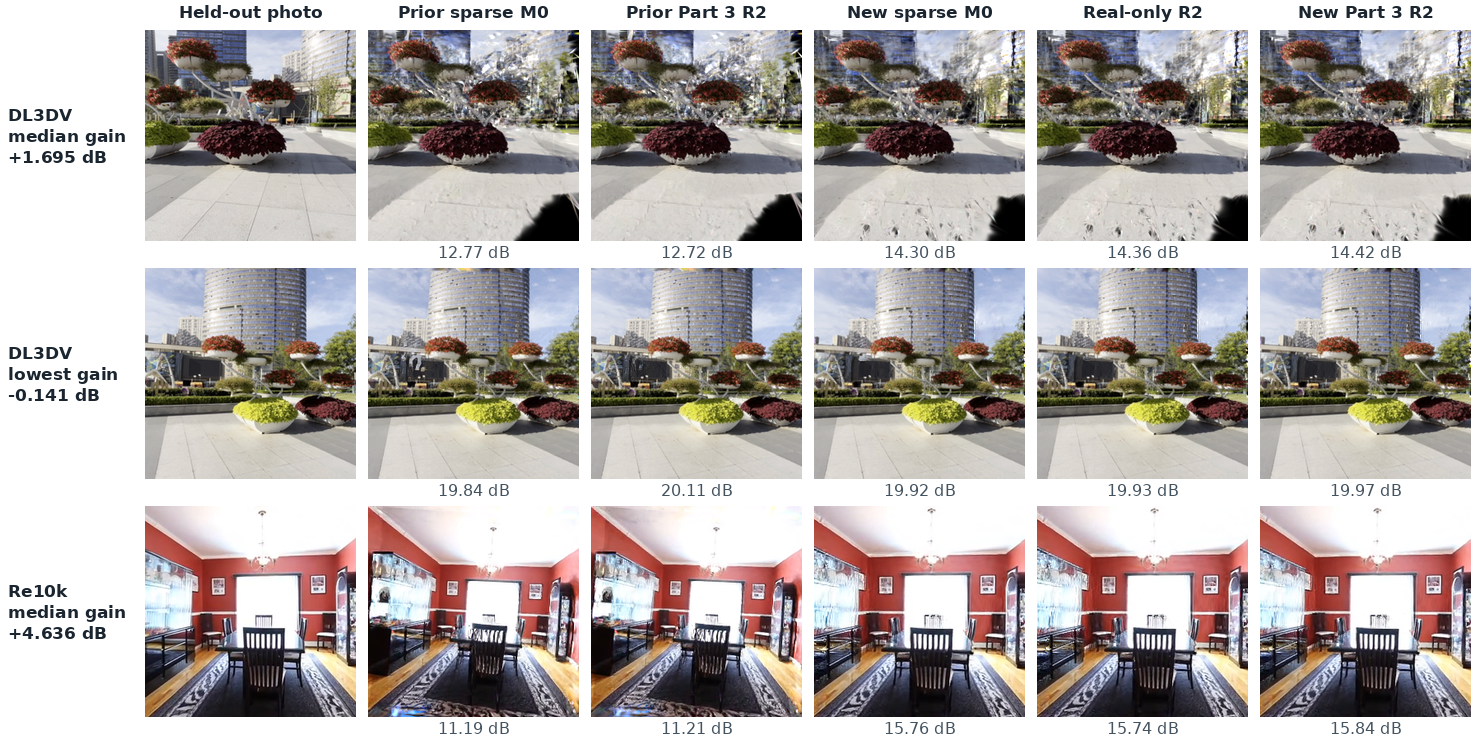
\includegraphics[width=0.93\textwidth]{../results/part3_mse30/heldout_comparison.png}
  \caption{Raw renders from the 13k texture-guided study at matched held-out viewpoints. Rows show the median and lowest PSNR gains on DL3DV and the median gain on Re10k relative to the earlier Part~3 result. The real-only column uses the same initialization and extra training budget.}
  \label{fig:loop_qual}
\end{figure*}
}

\newcommand{\partthreeresults}{%
\paragraph{Protocol.}
The course evaluation covers 29 scene states and 961 raw test renders across 99 distinct images. Replay of the Part 2 checkpoints matches archived metrics within $1.9\times10^{-6}$. Each round adds 3,000 updates, and augmented branches use four pseudo-views with $\lambda=0.2$. Difix-ref uses half precision, a maximum input edge of 768, and fixed seeds. We recompute view priorities from each round's parent scene (Fig.~\ref{fig:active_trajectory}).

\paragraph{Held-out quality and controls.}
Active gated round two improves PSNR by 0.019, 0.022, and 0.016~dB on Waymo, DL3DV, and Re10k relative to $M_0$, respectively (Table~\ref{tab:part3_main}, Fig.~\ref{fig:closed_loop}). PSNR gains over real-only are 0.041, 0.029, and 0.007~dB, with lower LPIPS in all three scenes. Final SSIM falls below $M_0$ throughout. DL3DV's round one improves all metrics over $M_0$ and has the largest PSNR gain, 0.041~dB. Waymo PSNR falls initially and exceeds $M_0$ after two diffusion rounds. Raw replay gives smaller gains on DL3DV and Re10k. Gating improves final PSNR over ungated diffusion by 0.0012--0.0054~dB and slightly worsens LPIPS.

\paragraph{Active versus fixed planning.}
On Re10k, fixed gated planning has higher PSNR in round one. Active gated planning leads by 0.0047~dB at the second round, while fixed planning retains a 0.00026 LPIPS advantage. The small changes and single-scene ablation leave the planner's benefit uncertain across scenes.

\paragraph{Generated views and failure cases.}
The Re10k targets in Fig.~\ref{fig:pseudo_views} have 96.9\% and 93.1\% reprojection support. Confidence falls near chair and window edges even when restoration changes their appearance. In Fig.~\ref{fig:loop_qual}, DL3DV frame 00001 gains 0.255~dB from $M_0$ to gated round two, and the real-only control reaches slightly higher PSNR on the same view. Waymo frame 000192 loses 0.180~dB despite lower LPIPS. Its vehicles and road edges remain blurred. The examples show why the scene-average gain and visual effects of restoration should be evaluated separately.

\paragraph{Cost of the closed loop.}
For the course scenes on the RTX A6000, active gated planning takes 0.15--5.39~s per round. Preparing four targets takes 1.73--18.13~s, including rendering, restoration, projection checks, and writes, excluding restorer loading. Gated optimization takes 115--213~s per round versus 76--153~s for real-only. The stage totals include restorer setup and evaluation. A transient GPU memory error during Waymo round-two restoration required a retry from the same checkpoint with identical settings.

\paragraph{Supplemental Bonsai scene.}
For Mip-NeRF 360 Bonsai~\cite{barron2022mipnerf360}, we hold out every eighth file in natural order (37 images) and sample 12 evenly spaced training images from the remainder. We fit an independent, VGGT-initialized 7,000-step $M_0$ from $512\times341$ training RGB. The released COLMAP cameras are used for evaluation. Baseline PSNR, SSIM, and LPIPS are 14.4350, 0.3172, and 0.4244. Active gated fusion improves all three metrics in round one. Its round-two PSNR is 0.004~dB above $M_0$ and 0.035~dB above real-only, with lower SSIM and higher LPIPS than $M_0$ (Table~\ref{tab:bonsai}).

\noindent\begin{minipage}{\columnwidth}
  \centering\footnotesize
  \setlength{\tabcolsep}{2.5pt}
  \begin{tabular}{@{}lcc@{}}
    \toprule
    Condition & Round 1 & Round 2 \\
    \midrule
    Real only & 14.4159 / .3143 / .4281 & 14.4037 / .3129 / .4312 \\
    Raw replay & 14.4370 / .3153 / .4267 & 14.4328 / .3142 / .4286 \\
    Ungated & 14.4609 / .3174 / .4220 & 14.4168 / .3147 / .4249 \\
    Gated & 14.4683 / .3174 / .4228 & 14.4386 / .3155 / .4251 \\
    \bottomrule
  \end{tabular}
  \captionof{table}{Bonsai test metrics as PSNR (dB) / SSIM / LPIPS.}
  \label{tab:bonsai}
\end{minipage}
}
